\noindent\textbf{Any}
\lstinputlisting[firstline=1,lastline=3]{transformations/bag/emftvm/TestAny.atl}
\begin{figure*}[h]
\centering
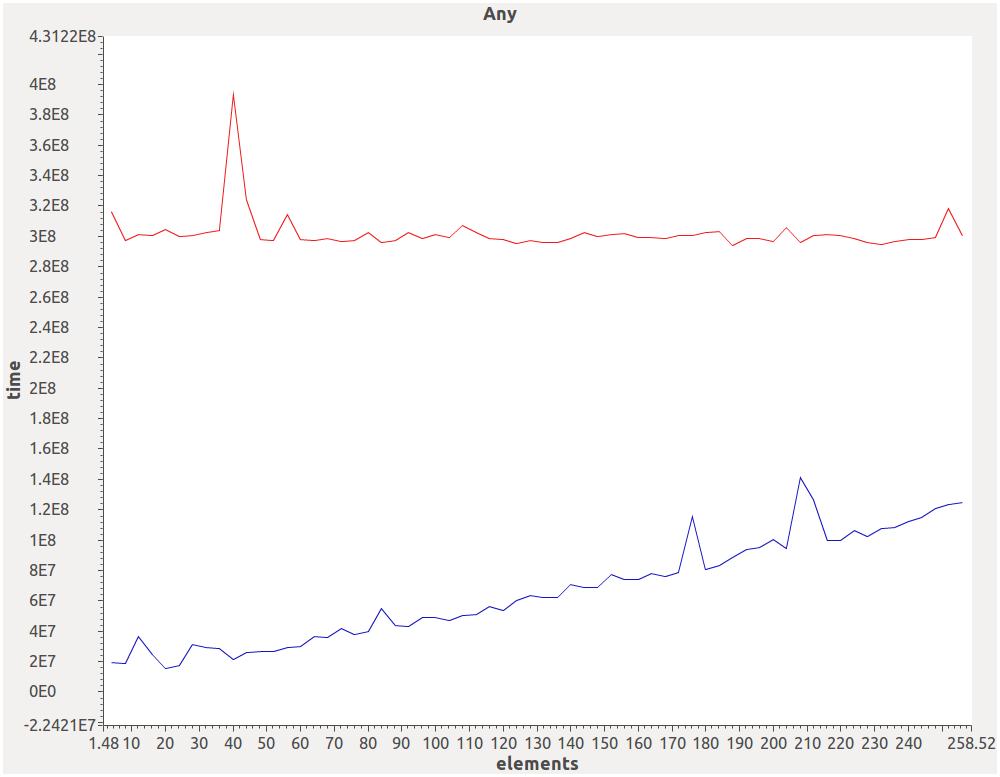
\includegraphics[width=\textwidth]{graphs/bag/Any}
\end{figure*}
\pagebreak

\noindent\textbf{Collect}
\lstinputlisting[firstline=1,lastline=3]{transformations/bag/emftvm/TestCollect.atl}
\begin{figure*}[h]
\centering
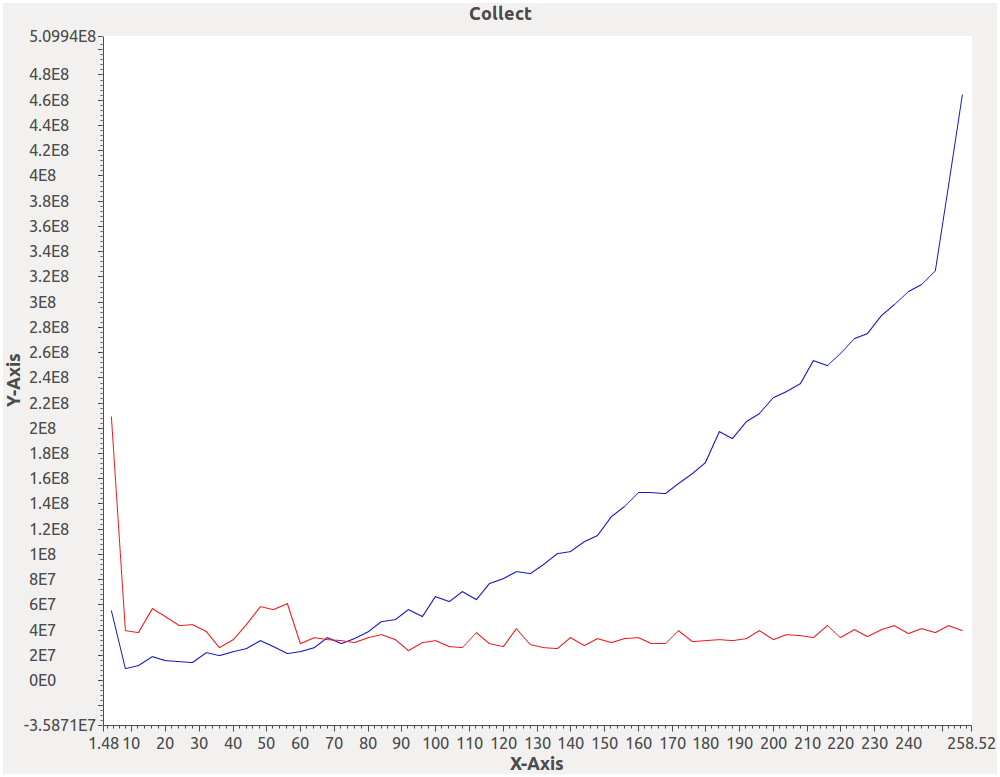
\includegraphics[width=\textwidth]{graphs/bag/Collect}
\end{figure*}
\pagebreak

\noindent\textbf{EQ}
\lstinputlisting[firstline=1,lastline=3]{transformations/bag/emftvm/TestEQ.atl}
\begin{figure*}[h]
\centering
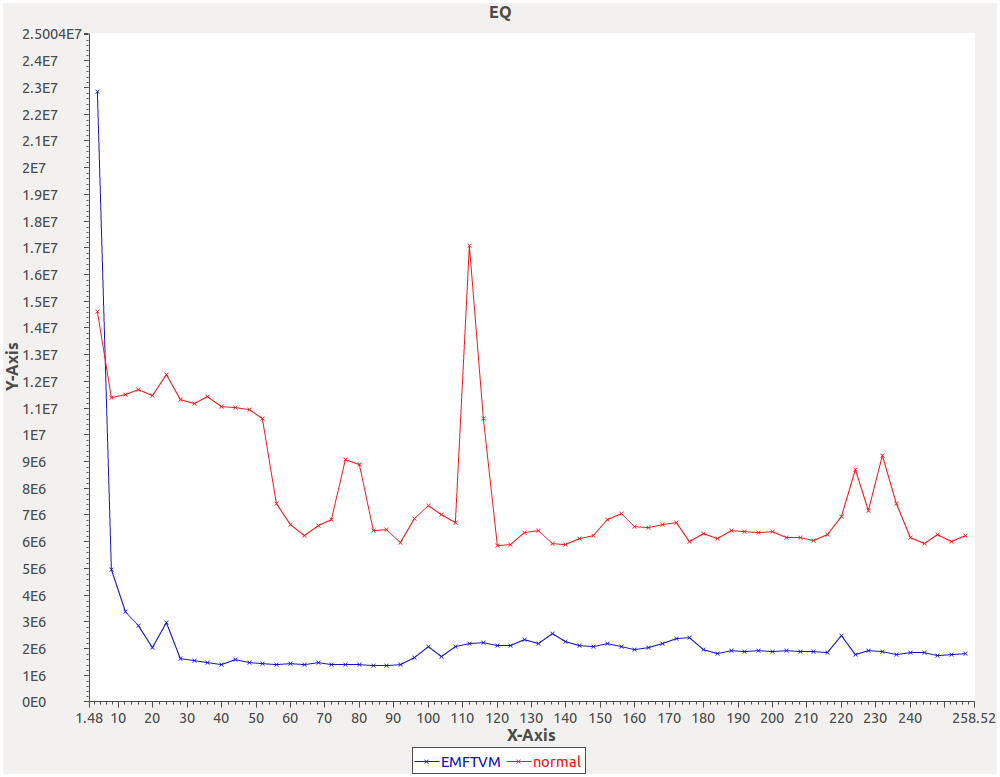
\includegraphics[width=\textwidth]{graphs/bag/EQ}
\end{figure*}
\pagebreak

\noindent\textbf{Excludes}
\lstinputlisting[firstline=1,lastline=3]{transformations/bag/emftvm/TestExcludes.atl}
\begin{figure*}[h]
\centering
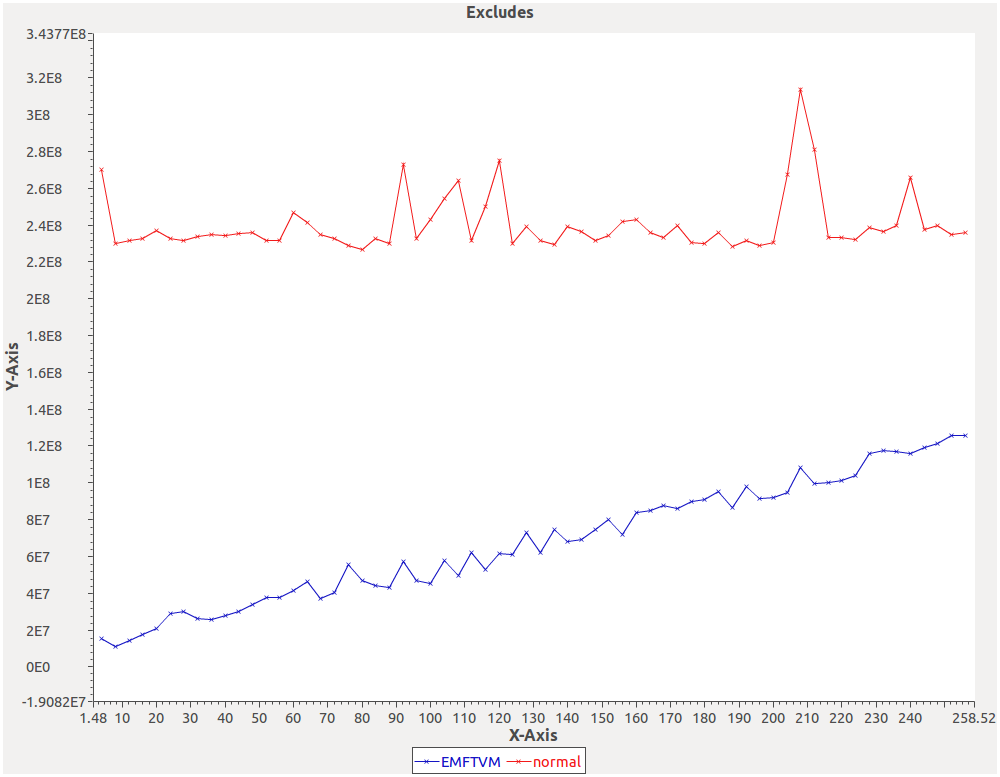
\includegraphics[width=\textwidth]{graphs/bag/Excludes}
\end{figure*}
\pagebreak

\noindent\textbf{ExcludesAll}
\lstinputlisting[firstline=1,lastline=3]{transformations/bag/emftvm/TestExcludesAll.atl}
\begin{figure*}[h]
\centering
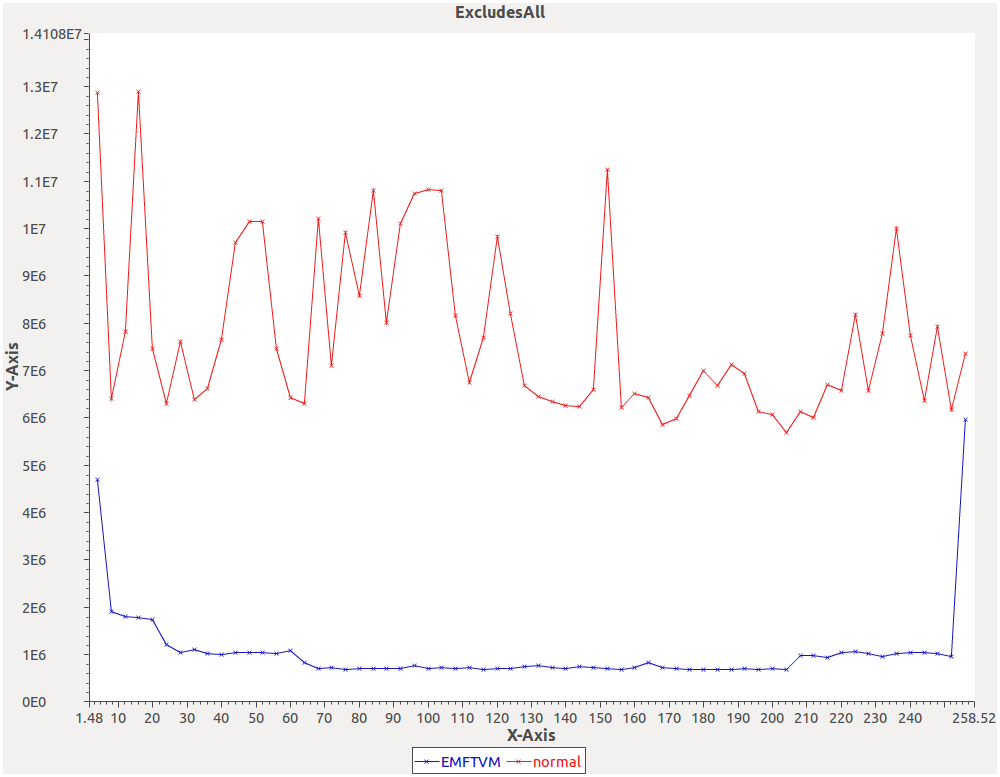
\includegraphics[width=\textwidth]{graphs/bag/ExcludesAll}
\end{figure*}
\pagebreak

\noindent\textbf{Excluding}
\lstinputlisting[firstline=1,lastline=3]{transformations/bag/emftvm/TestExcluding.atl}
\begin{figure*}[h]
\centering
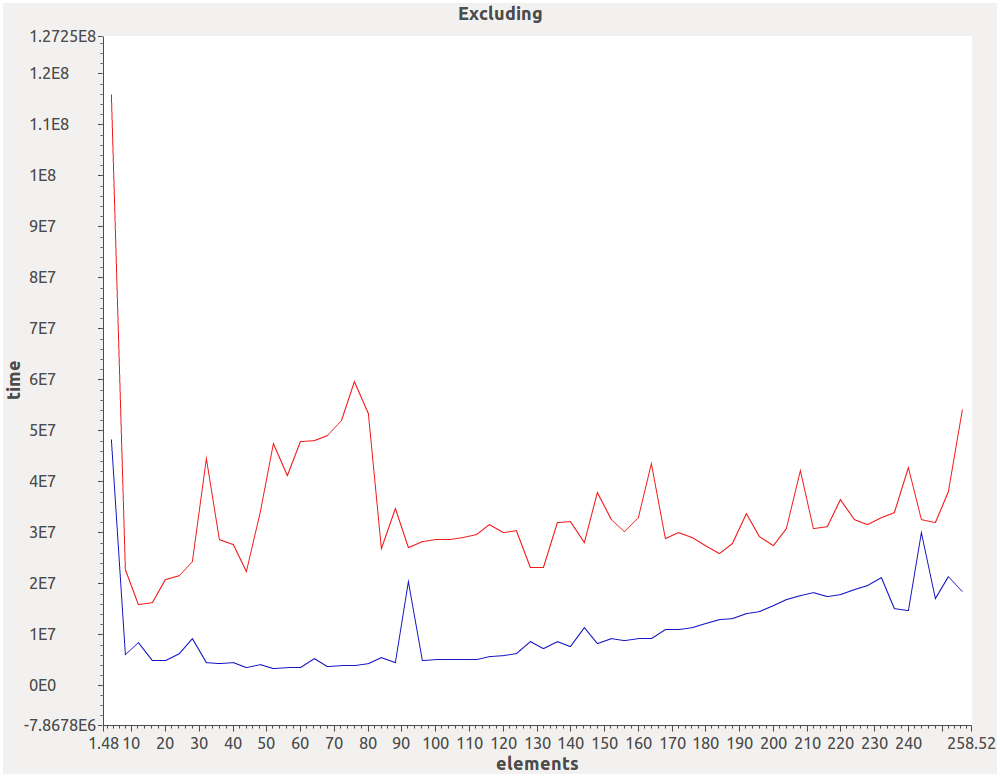
\includegraphics[width=\textwidth]{graphs/bag/Excluding}
\end{figure*}
\pagebreak

\noindent\textbf{Exists}
\lstinputlisting[firstline=1,lastline=3]{transformations/bag/emftvm/TestExists.atl}
\begin{figure*}[h]
\centering
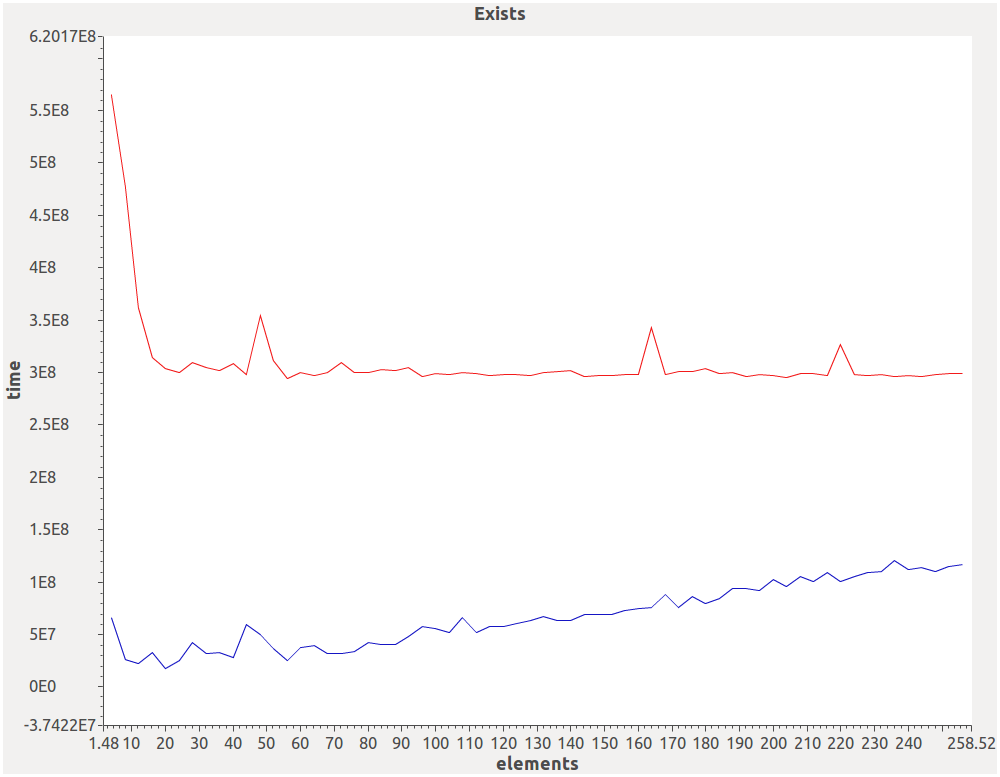
\includegraphics[width=\textwidth]{graphs/bag/Exists}
\end{figure*}
\pagebreak

\noindent\textbf{Flatten}
\lstinputlisting[firstline=1,lastline=3]{transformations/bag/emftvm/TestFlatten.atl}
\begin{figure*}[h]
\centering
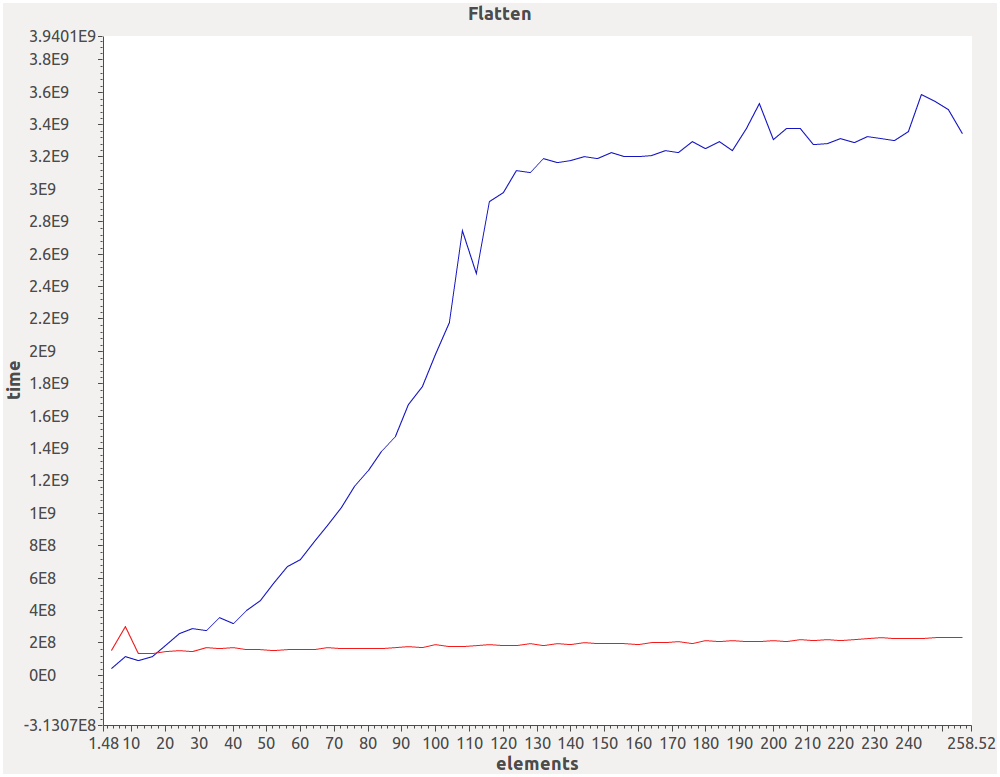
\includegraphics[width=\textwidth]{graphs/bag/Flatten}
\end{figure*}
\pagebreak

\noindent\textbf{ForAll}
\lstinputlisting[firstline=1,lastline=3]{transformations/bag/emftvm/TestForAll.atl}
\begin{figure*}[h]
\centering
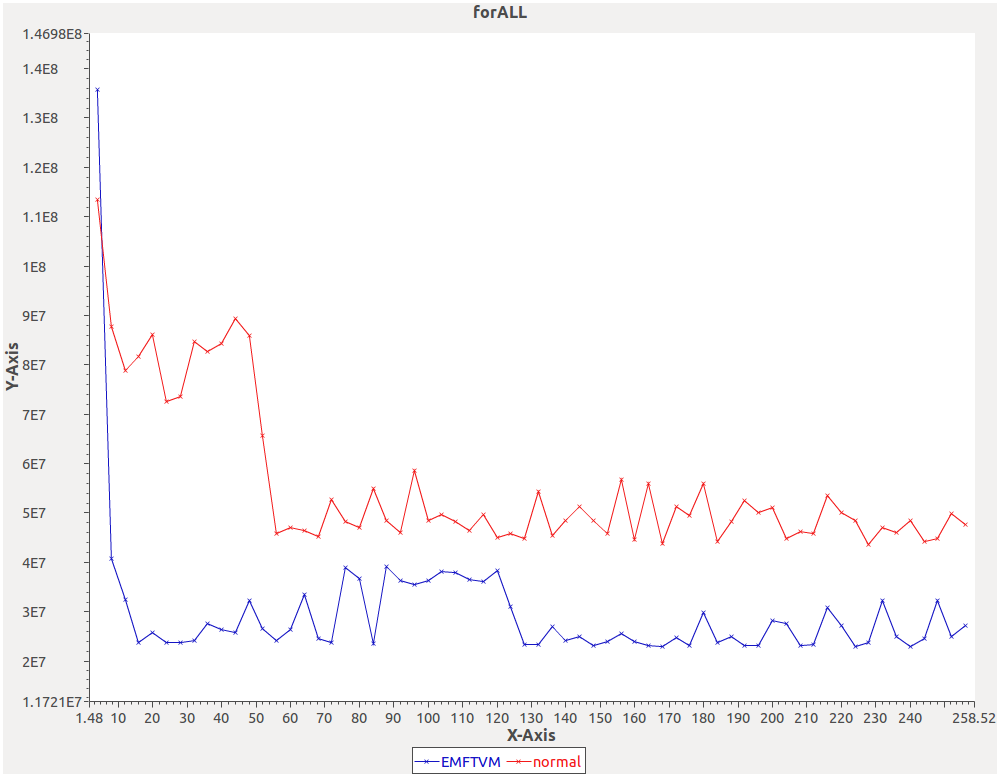
\includegraphics[width=\textwidth]{graphs/bag/forALL}
\end{figure*}
\pagebreak

\noindent\textbf{Includes}
\lstinputlisting[firstline=1,lastline=3]{transformations/bag/emftvm/TestIncludes.atl}
\begin{figure*}[h]
\centering
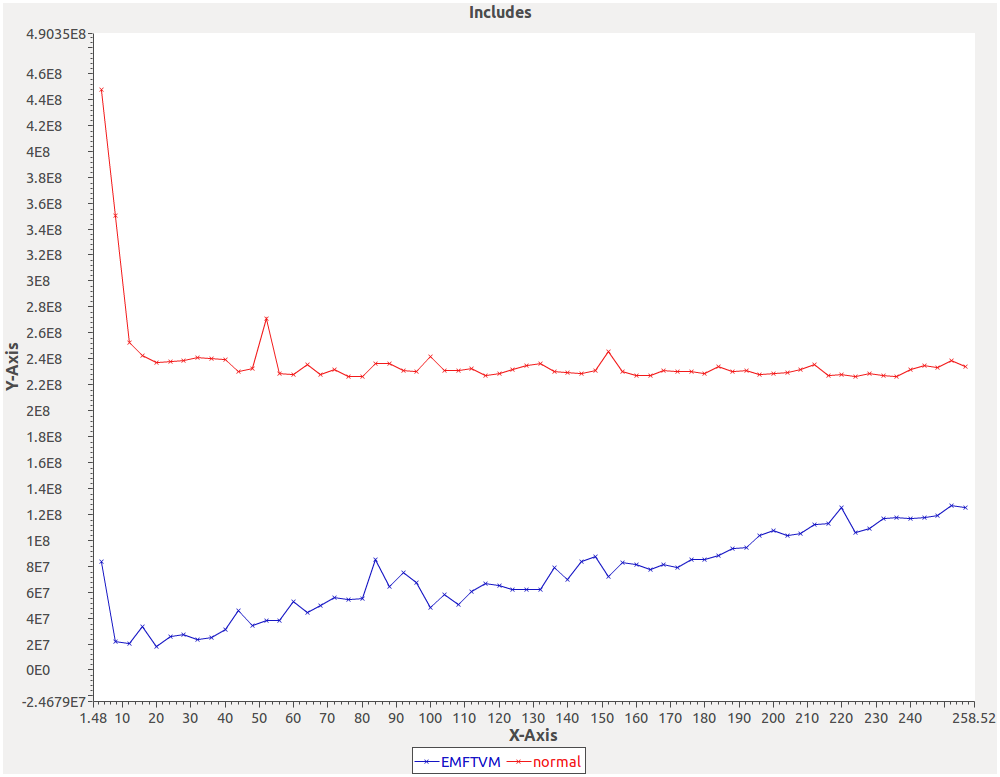
\includegraphics[width=\textwidth]{graphs/bag/Includes}
\end{figure*}
\pagebreak

\noindent\textbf{IncludesAll}
\lstinputlisting[firstline=1,lastline=3]{transformations/bag/emftvm/TestIncludesAll.atl}
\begin{figure*}[h]
\centering
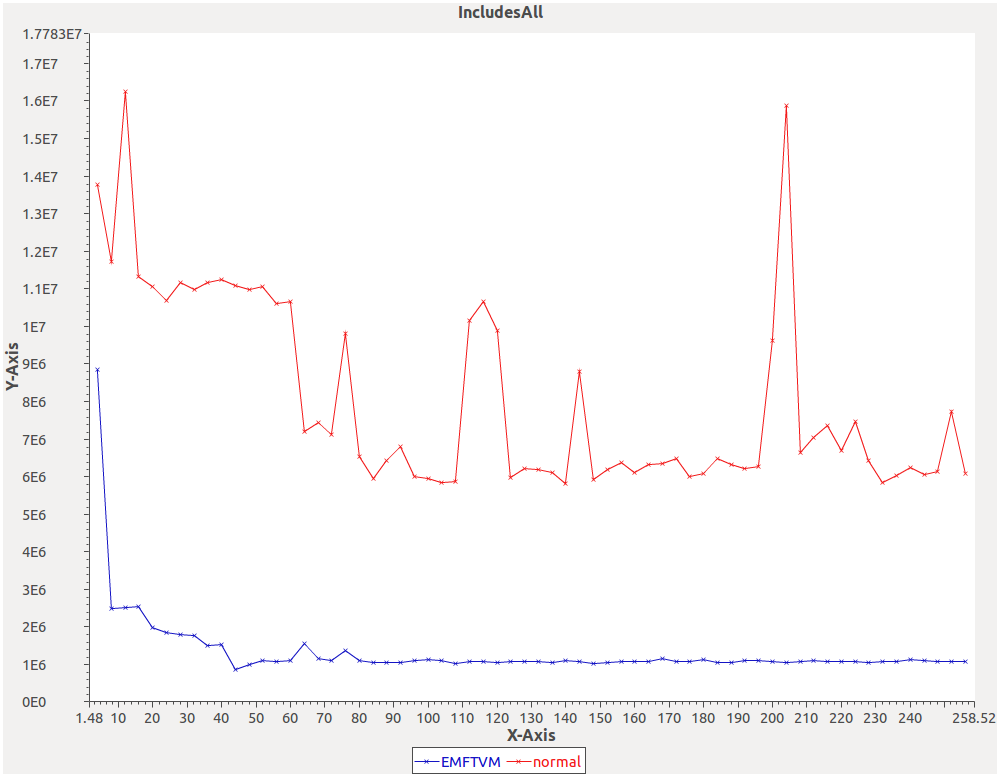
\includegraphics[width=\textwidth]{graphs/bag/IncludesAll}
\end{figure*}
\pagebreak

\noindent\textbf{Including}
\lstinputlisting[firstline=1,lastline=3]{transformations/bag/emftvm/TestIncluding.atl}
\begin{figure*}[h]
\centering
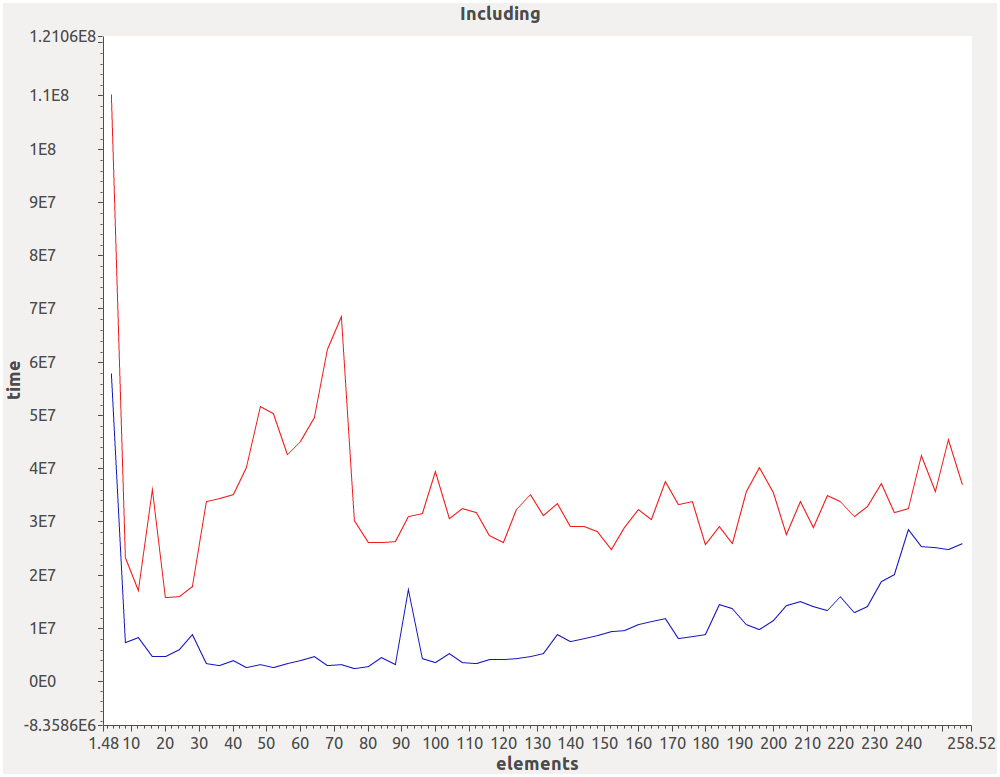
\includegraphics[width=\textwidth]{graphs/bag/Including}
\end{figure*}
\pagebreak

\noindent\textbf{IsEmpty}
\lstinputlisting[firstline=1,lastline=3]{transformations/bag/emftvm/TestIsEmpty.atl}
\begin{figure*}[h]
\centering
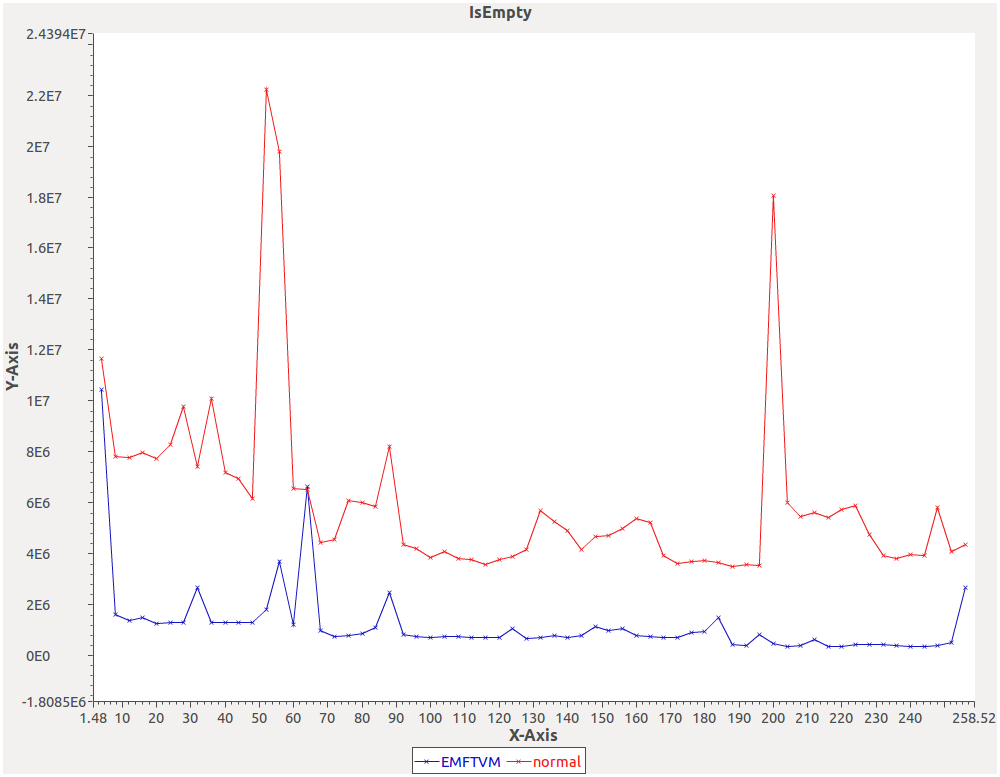
\includegraphics[width=\textwidth]{graphs/bag/IsEmpty}
\end{figure*}
\pagebreak

\noindent\textbf{IsUnique}
\lstinputlisting[firstline=1,lastline=3]{transformations/bag/emftvm/TestIsUnique.atl}
\begin{figure*}[h]
\centering
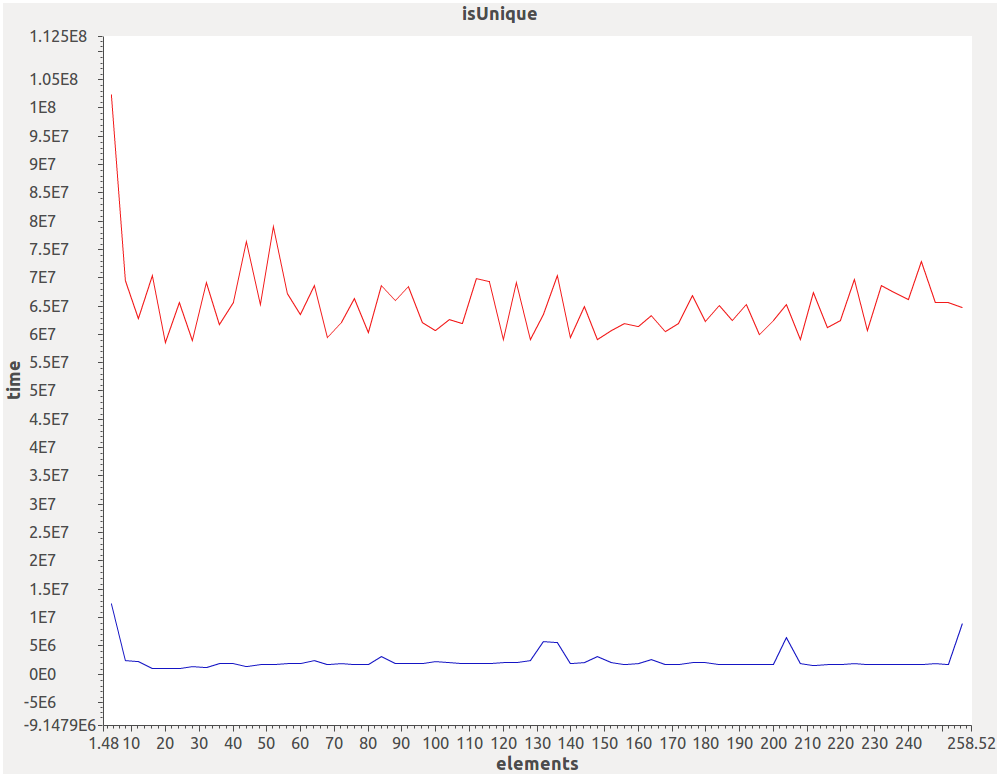
\includegraphics[width=\textwidth]{graphs/bag/isUnique}
\end{figure*}
\pagebreak

\noindent\textbf{Iterate}
\lstinputlisting[firstline=1,lastline=3]{transformations/bag/emftvm/TestIterate.atl}
\begin{figure*}[h]
\centering
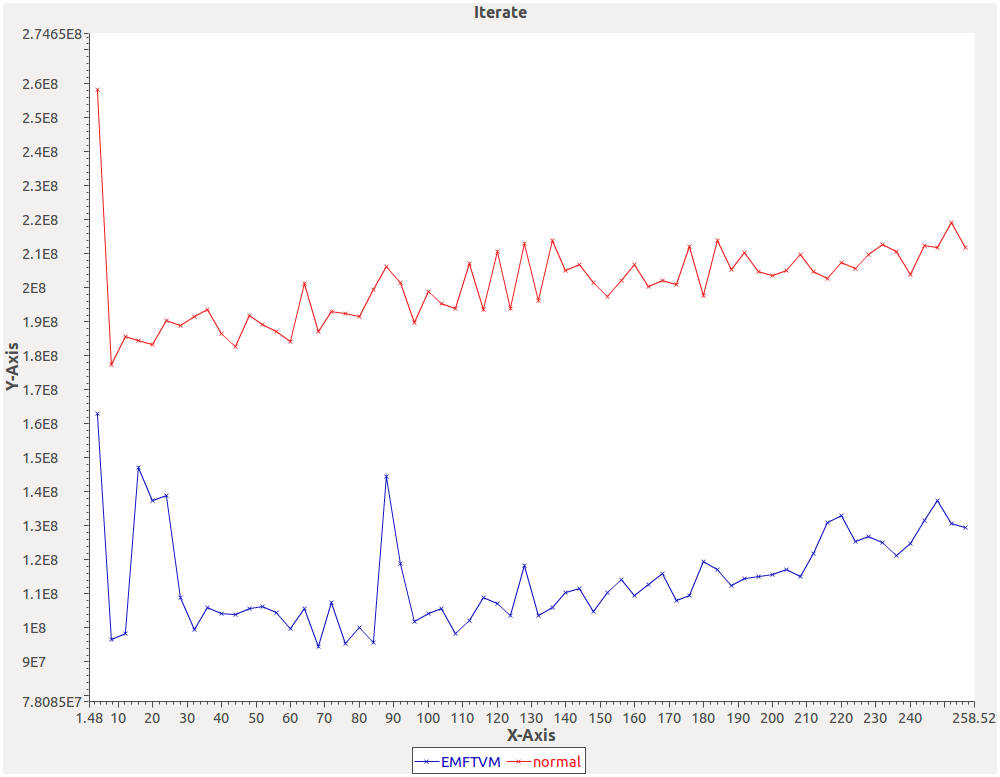
\includegraphics[width=\textwidth]{graphs/bag/Iterate}
\end{figure*}
\pagebreak

\noindent\textbf{NotEqual}
\lstinputlisting[firstline=1,lastline=3]{transformations/bag/emftvm/TestNeq.atl}
\begin{figure*}[h]
\centering
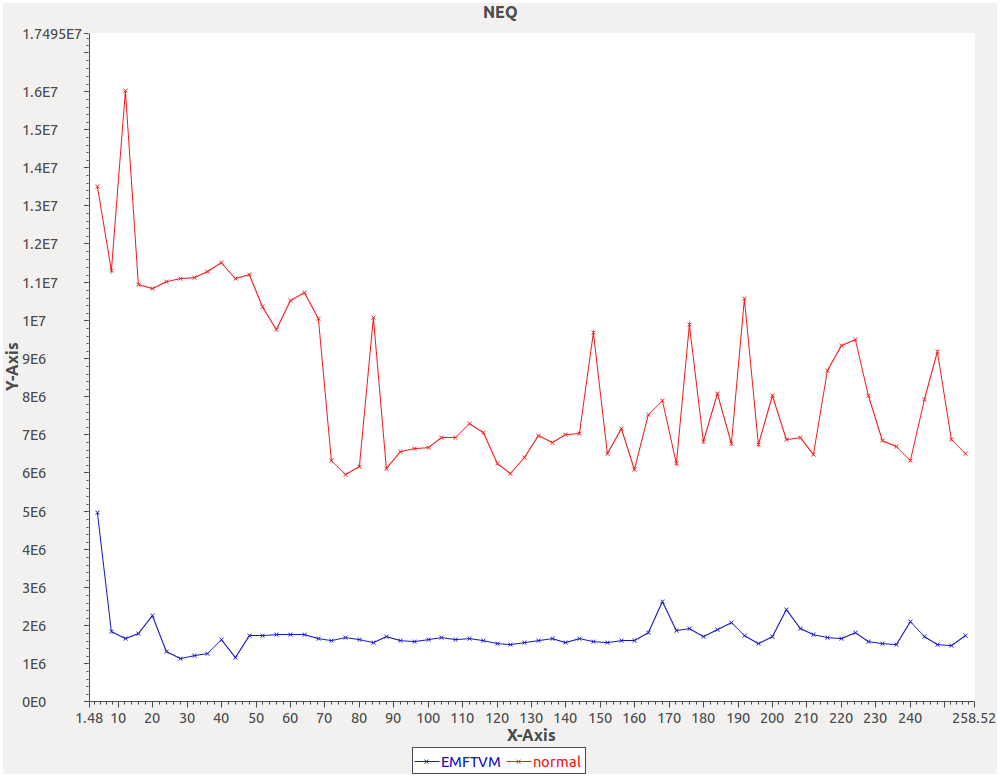
\includegraphics[width=\textwidth]{graphs/bag/NEQ}
\end{figure*}
\pagebreak

\noindent\textbf{One}
\lstinputlisting[firstline=1,lastline=3]{transformations/bag/emftvm/TestOne.atl}
\begin{figure*}[h]
\centering
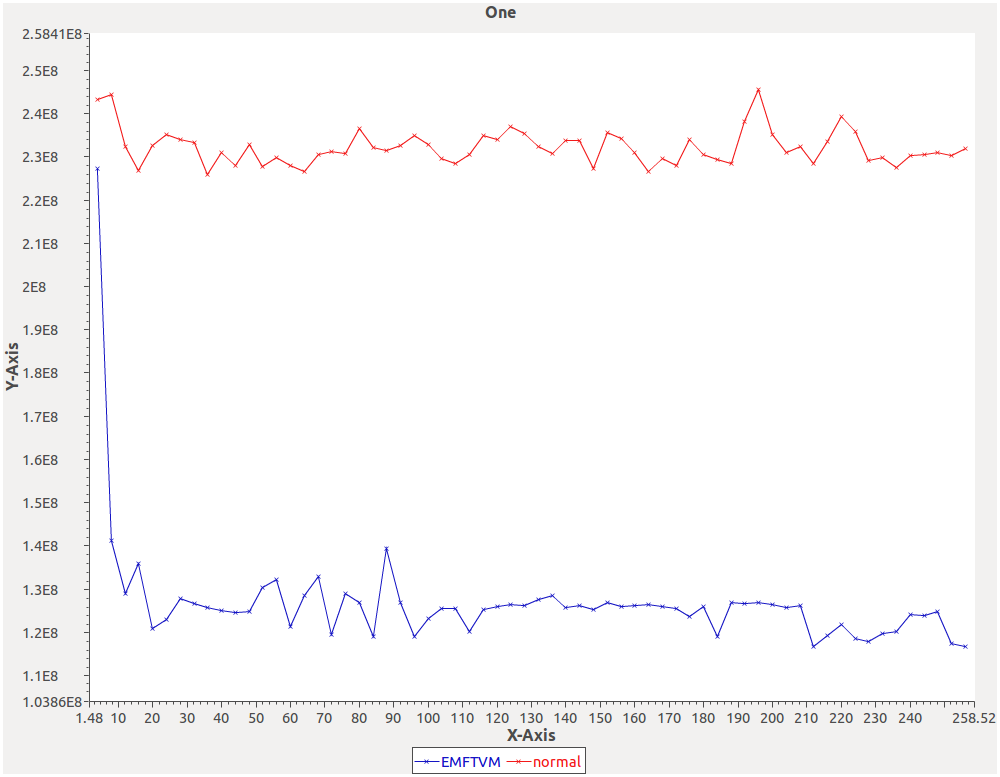
\includegraphics[width=\textwidth]{graphs/bag/One}
\end{figure*}
\pagebreak

\noindent\textbf{Reject}
\lstinputlisting[firstline=1,lastline=3]{transformations/bag/emftvm/TestReject.atl}
\begin{figure*}[h]
\centering
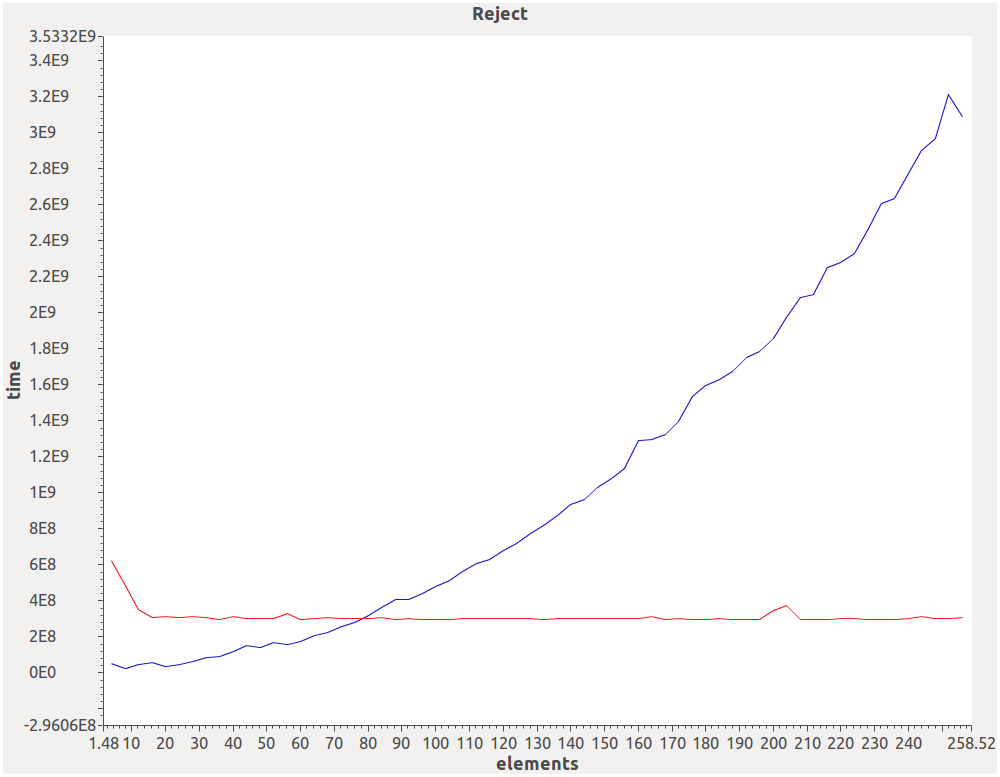
\includegraphics[width=\textwidth]{graphs/bag/Reject}
\end{figure*}
\pagebreak

\noindent\textbf{Select}
\lstinputlisting[firstline=1,lastline=3]{transformations/bag/emftvm/TestSelect.atl}
\begin{figure*}[h]
\centering
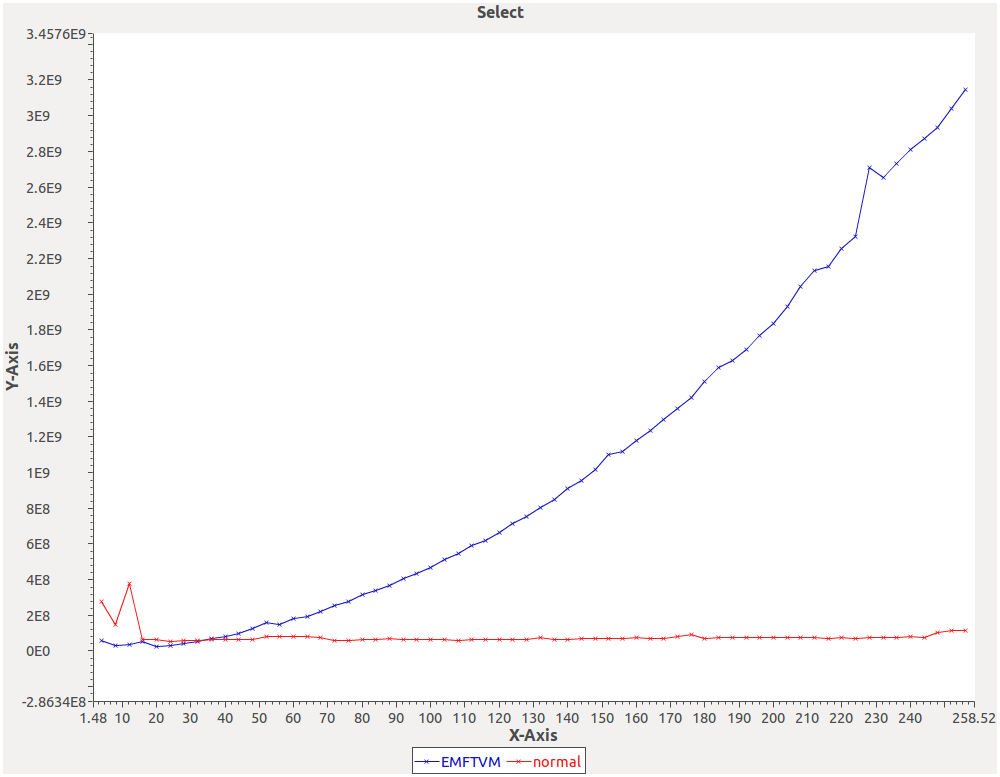
\includegraphics[width=\textwidth]{graphs/bag/Select}
\end{figure*}
\pagebreak

\noindent\textbf{Size}
\lstinputlisting[firstline=1,lastline=3]{transformations/bag/emftvm/TestSize.atl}
\begin{figure*}[h]
\centering
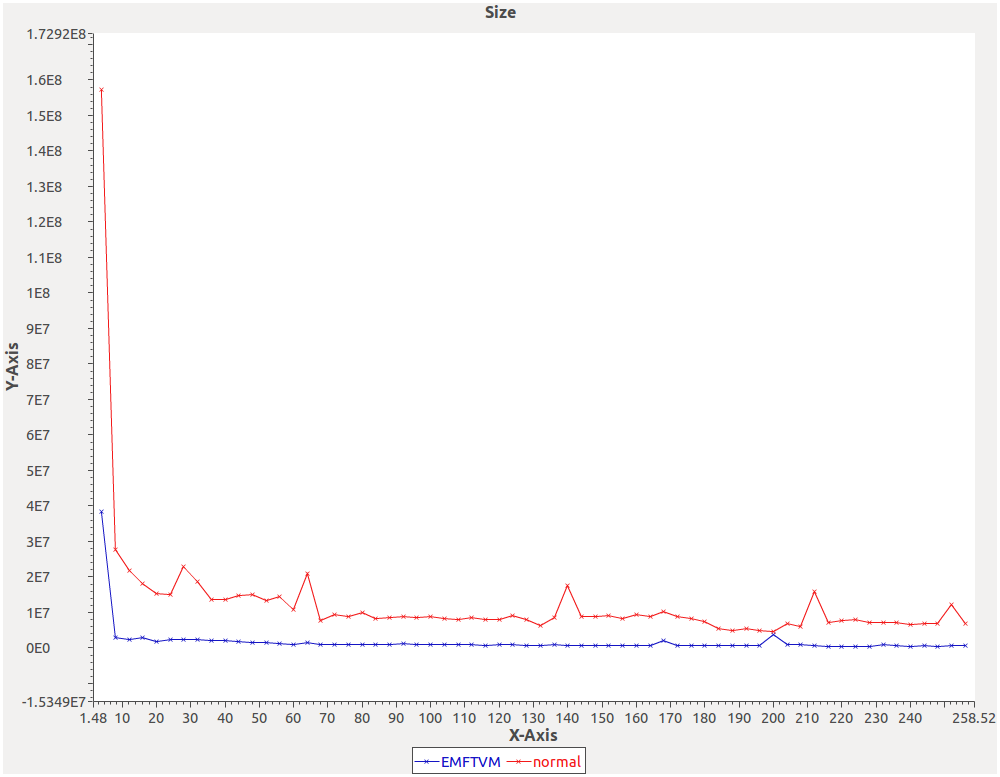
\includegraphics[width=\textwidth]{graphs/bag/Size}
\end{figure*}
\pagebreak

\noindent\textbf{SortedBy}
\lstinputlisting[firstline=1,lastline=3]{transformations/bag/emftvm/TestSortedBy.atl}
\begin{figure*}[h]
\centering
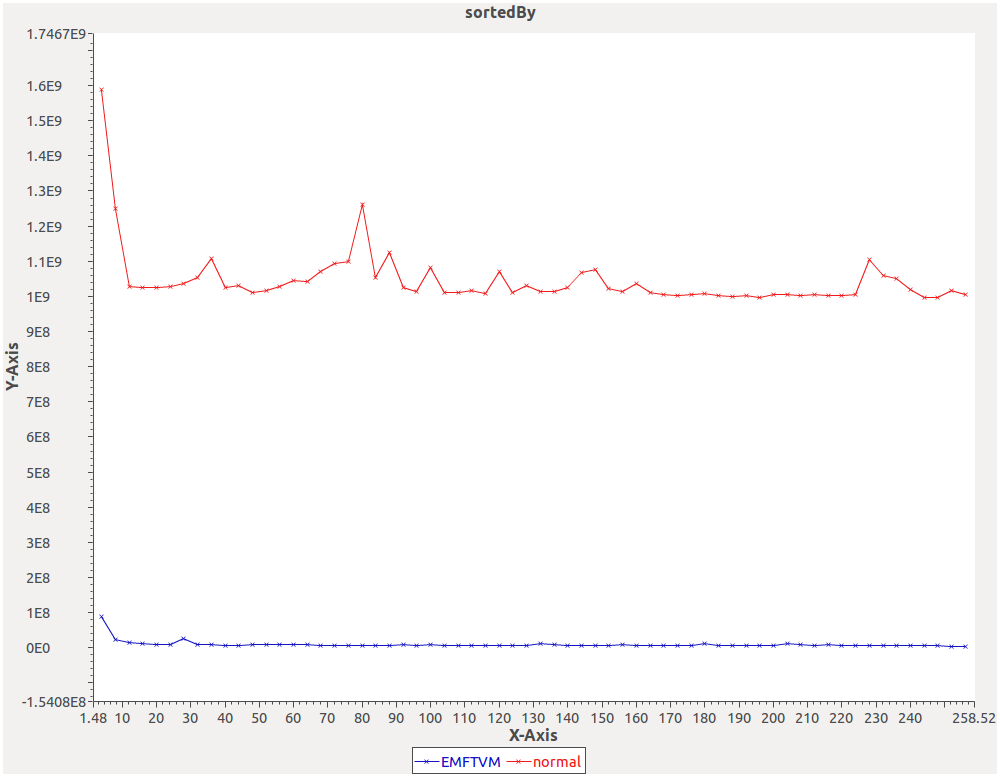
\includegraphics[width=\textwidth]{graphs/bag/sortedBy}
\end{figure*}e
\pagebreak

\noindent\textbf{Sum}
\lstinputlisting[firstline=1,lastline=3]{transformations/bag/emftvm/TestSum.atl}
\begin{figure*}[h]
\centering
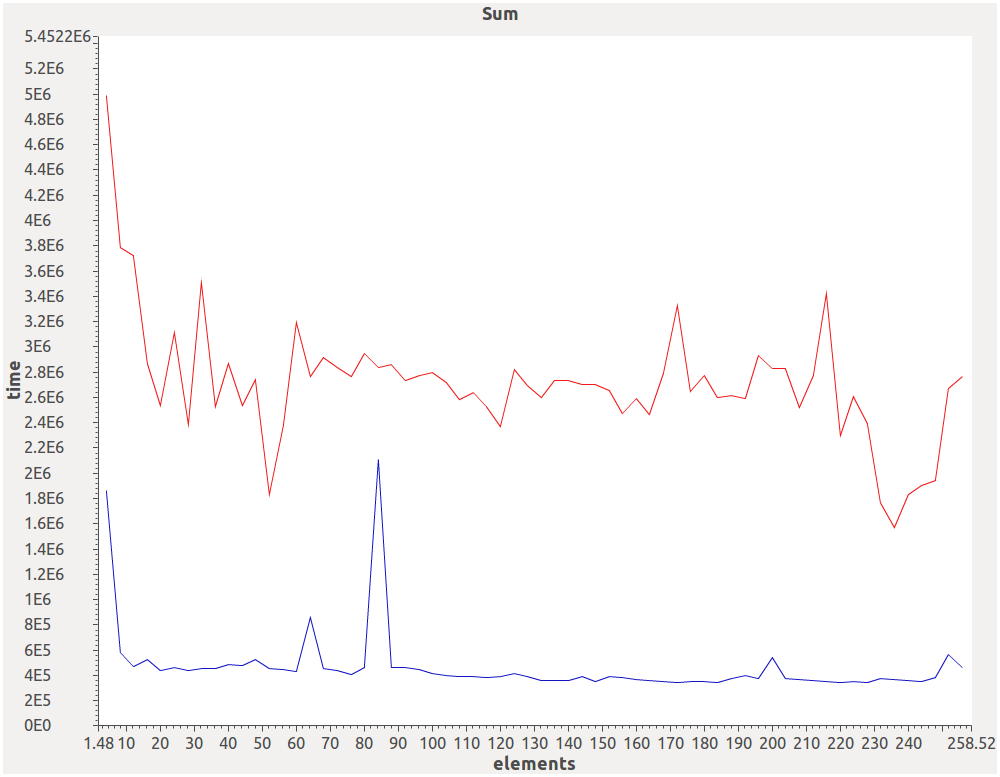
\includegraphics[width=\textwidth]{graphs/bag/Sum}
\end{figure*}
\pagebreak
